\chapter{Asking Texan Billionaires How They Got Rich!}

These notes follow a School of Hard Knocks interview episode, curated by LazyingArt LLC, and read it as a lecture on commercial scale. The host does not proceed by abstract thesis. He begins with spectacle, pauses to tell us why Texas is the right field in which to search, and then repeatedly converts visible wealth into a question of mechanism. The mathematics is therefore schematic rather than technical, but the lecture is rich in quantities, comparisons, allocations, and decision structures, and those are what we preserve.

\section{Texas as a Wealth Field}

The lecture opens with a cold proof of access. Before we are told what Texas means, we are shown what the host can reach: a G-Wagon owner in software and investing, a founder tied to Venmo, a business doing hundreds of millions in revenue, and another operator speaking of companies doing more than a billion dollars each year. The order matters. First we are shown scale; only then are we told why the scale is not accidental.

The opening numerical bank is therefore not decoration. It is the host's way of certifying the field:
\begin{align}
S_{\mathrm{sale}} &\approx \$800\times 10^{6},\\
R_{\mathrm{company}} &> \$850\times 10^{6},\\
R_{\mathrm{founded\ companies}} &> \$1\times 10^{9}\ \text{per year}.
\end{align}

The host then widens the lens from anecdote to geography:
\begin{align}
N_{\mathrm{TX,billionaires}} &> 80,\\
\operatorname{rank}_{\mathrm{economy}}(\mathrm{Texas}) &= 8.
\end{align}

Once those statements are in place, Austin stops being scenery. It becomes what we might call a wealth field: a region dense enough in capital, exits, and ambitious operators that the host can ask the same set of questions over and over and expect instructive variation rather than noise. This is the first structural beat of the lecture. We choose the field first; only then do we ask what kinds of engines are running inside it.

\section{Action, Responsibility, and the First Wealth Machine}

The first long stop is with the smoothie entrepreneur. This is the lecture's first decisive pivot away from visible outcomes and toward the moral mechanics of commercial life. The speaker gives two revenue anchors,
\begin{equation}
R_{\mathrm{smoothie,last}} \approx \$23\times 10^{6},
\qquad
R_{\mathrm{smoothie,this}} \in [\$32,\$35]\times 10^{6},
\end{equation}
and that matters because it keeps the discussion from floating off into unsupported exhortation. These are not merely attitudes attached to no business at all; they are attitudes attached to a measurable enterprise.

The host then asks the right threshold question: is everybody built for entrepreneurship? The answer is given in deliberately harsh, almost primitive language, and we can compress it as
\begin{equation}
\mathcal{P}=\{\text{talkers},\ \text{doers}\}.
\end{equation}

This partition is not offered as sociology. It is offered as a filter. The lecture wants us to understand that, before we speak of market selection or strategic leverage, we must speak of a much blunter separation: the person who moves and the person who stalls.

\subsection{Question \& Answer}

\paragraph{Question.} What actually separates wanting entrepreneurship from being built for it?

\paragraph{Answer.} In this lecture it is not talent in the abstract, and not pedigree, and not the right buzzword. The answer is a sequence of practical and moral moves under pressure. The speaker begins with action, but he does not leave us there. He immediately drives the point inward: surrender, responsibility, work, thrift, investment.

That sequence may be written in the lecture's own spirit as
\begin{equation}
\text{surrender}
\to
\text{responsibility}
\to
\text{labor}
\to
\text{saving}
\to
\text{investing}.
\end{equation}

The transcript strengthens this chain by giving us the prior state in detail: victimhood, blame, addiction, homelessness, and years spent narrating the self as damaged by others. The turning point is therefore not a tip but a reassignment of causality. Once the speaker ceases to place cause elsewhere, action becomes available again.

A minimal financial expression of that logic is
\begin{equation}
\text{income}-\text{spending}>0
\quad\Longrightarrow\quad
\text{savings}>0
\quad\Longrightarrow\quad
\text{investment capacity}>0.
\end{equation}

By itself this is trivial arithmetic. Inside the lecture it is not trivial, because it is attached to biography. The arithmetic is the outer shell of a deeper transformation in agency.

The interview closes with an unexpected but necessary seal: take care of one's mother, take care of family, do not let business ambition sever duty. That is not a separate theme tacked on at the end. It is the lecture's first reminder that scale without order in the person is not the kind of success this episode wants to celebrate. The host then steps out and recaps the conversation in exactly that way: the smoothie business may do roughly thirty million this year, but the real payload of the encounter is the hierarchy of responsibility that carried it.

\section{Mispriced Opportunity and the Geography of Capital}

The next movement changes scale again. We go from the reconstruction of a single operator to a statement about where opportunity is hiding in the world. The host asks for the best industry. The answer is framed as a deliberate correction of the question itself: not an industry in the narrow sense, but a geography, namely Africa.

The argument rests on a contrast between growth share and capital share. The speaker's numerical claims can be stored compactly as
\begin{align}
g_{\mathrm{Africa}} &= \frac{9}{20},\\
\alpha_{\mathrm{Africa}} &\approx 0.5\%.
\end{align}

Here \(g_{\mathrm{Africa}}\) is the claimed share of the twenty fastest-growing economies in 2025, while \(\alpha_{\mathrm{Africa}}\) is the claimed share of global private equity and venture capital flowing into Africa. The lecture does not pretend that these are identical quantities. The force lies in the mismatch. Growth, demography, digital leapfrogging, and labor energy are all placed on one side; very little incoming capital is placed on the other.

\subsection{Question \& Answer}

\paragraph{Question.} How can a geography function like an industry-level opportunity?

\paragraph{Answer.} Because the lecture is not trying to preserve categories for their own sake. It is trying to identify what capital systematically overlooks. If a region combines growth, a young and expanding population, and a technological pathway that skips old infrastructure, then it can behave, from the investor's point of view, like an underfunded domain of entrepreneurship. The point is not taxonomic correctness; the point is that markets often inherit bad labels and then allocate badly under those labels.

The transcript then enters a damaged stretch around a scaling anecdote. We should resist the temptation to over-formalize what the text no longer reliably gives us. Still, a clean operational principle survives:
\begin{equation}
\text{care for employees}
\to
\text{better service to customers}
\to
\text{better ideas}
\to
\text{stronger business}.
\end{equation}

That surviving line is enough to carry us into the next section. The lecture has now moved from mispriced geography to the social interior of the firm.

\section{The Hidden Team Behind the Visible Channel}

At precisely the point where a viewer might begin to romanticize individual stars, the host interrupts the flow and performs a correction on his own brand. He tells us that the channel's growth did not happen because of him alone. He names co-founders, editors, videographers, and strategists, and the selected frame makes that correction visible by turning the channel into a small role-stack diagram.

\begin{figure}
\centering

\includegraphics[width=0.78\textwidth]{lecture_43_figure_02.png}
\end{figure}

There is no board mathematics in this frame. What it gives us instead is evidentiary structure. From the icon stack alone we may cautiously write
\begin{equation}
\mathcal{T}_{\mathrm{visible}}=\{\text{people/team},\ \text{editing},\ \text{camera}\},
\end{equation}
while the spoken line enlarges this to
\begin{equation}
\mathcal{T}_{\mathrm{spoken}}
=
\{\text{co-founders},\ \text{editors},\ \text{videographers},\ \text{strategists}\}.
\end{equation}

The distinction between these two sets should be preserved. The first is visually supported; the second is transcript-supported. The gap is small but important.

A cleaned organizational sketch reads as follows:

\begin{figure}
\centering
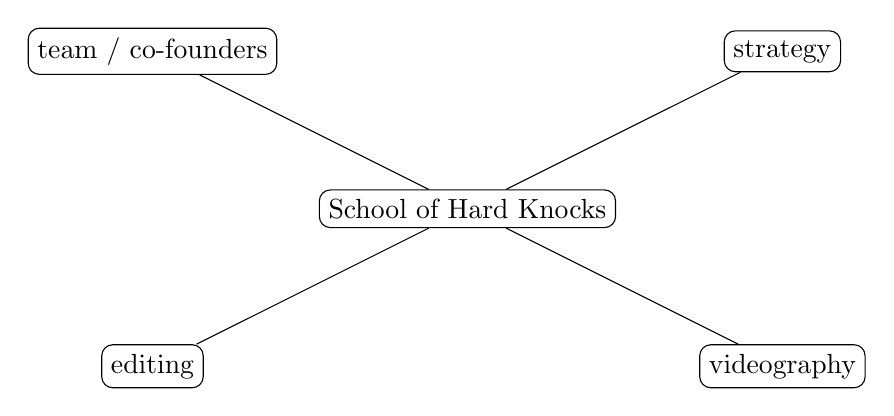
\begin{tikzpicture}
\node[draw, rounded corners] (s) at (0,0) {School of Hard Knocks};
\node[draw, rounded corners] (t) at (-4,2) {team / co-founders};
\node[draw, rounded corners] (e) at (-4,-2) {editing};
\node[draw, rounded corners] (v) at (4,-2) {videography};
\node[draw, rounded corners] (r) at (4,2) {strategy};
\draw (t) -- (s);
\draw (e) -- (s);
\draw (v) -- (s);
\draw (r) -- (s);
\end{tikzpicture}
\end{figure}

\subsection{Question \& Answer}

\paragraph{Question.} Why does the lecture stop to diagram the host's own team?

\paragraph{Answer.} Because the episode has reached a dangerous point. After enough encounters with wealthy individuals, the viewer may begin to attribute everything to the visible speaker. The host's team interlude breaks that illusion. It says that production is organizational even when the narrative surface is personal. In that sense the ZipRecruiter sponsor that follows is not a thematic interruption. It is a practical continuation of the same proposition: if team quality is part of the mechanism of scale, then hiring is not an afterthought but a structural business problem.

The host's own audience numbers are reported at slightly different levels across the lecture, and the right way to record them is as an approximate band:
\begin{equation}
F_{\mathrm{host}} \approx 12\times 10^{6}\ \text{to}\ 13\times 10^{6}.
\end{equation}

Again we do not fetishize exactness. The important thing is that even this scale is presented as distributed output rather than solitary genius.

\section{Health as Throughput, Not Ornament}

The Brian Johnson interview begins in a familiar way: exit size, business fame, the path into entrepreneurship. But then the lecture performs another of its self-corrections. Instead of asking immediately for the next business tactic, the host asks for the best advice, and the answer is: make health the number one life priority.

This is a local reframing of entrepreneurship itself. The business is still there, but the bottleneck is relocated from capital or market to the body and mind that must sustain the enterprise. The lecture's operational chain is therefore
\begin{equation}
\text{sleep and health priority}
\to
\text{clearer thinking}
\to
\text{better entrepreneurial decisions}.
\end{equation}

Johnson then extends the claim into a more radical zone. Because the lecture itself treats these as self-reported claims, we preserve them in exactly that register:
\begin{align}
a_{\mathrm{chronological}} &= 47,\\
a_{\mathrm{biological}} &\approx 18,\\
N_{\mathrm{rejuvenation}} &\approx 5000,\\
T_{\mathrm{birthday}} &\approx 24\ \text{months}.
\end{align}

\begin{remark}
The quantities in this section are speaker-attributed and should remain so. They help us understand the logic of the interview, but they are not to be silently upgraded into neutral scientific statements.
\end{remark}

\subsection{Question \& Answer}

\paragraph{Question.} Can health be a higher-yield business input than more grind?

\paragraph{Answer.} In the logic of this lecture, yes. The comparison is not between health and seriousness; it is between health and degraded throughput. If sleep loss, poor biomarkers, and chronic strain make thought fuzzy, then ``more effort'' may produce less value. Health is therefore cast not as a leisure good but as a multiplier on judgment.

The interview then deliberately enlarges itself. What begins as a correction of entrepreneurial culture widens into claims about slower aging, longer horizons, and even the possibility of dramatically expanded lifespan. That widening should remain in the notes because it is part of the lecture's rhythm. The host does not merely collect business rules; he repeatedly lets a practical question open out into a larger view of what human ambition might mean.

A second chain survives from this part of the lecture:
\begin{equation}
\text{slower aging}
\to
\text{more available time}
\to
\text{more room for technological rescue}.
\end{equation}

That chain is speculative, but it is the speculative edge of the interview, and it leads directly to the host's own recap: we thought we were talking about wealth, and suddenly we were talking about the more primary condition under which wealth can even matter, namely health.

\section{The 90/10 Rule}

The final software founder restores the lecture to its clearest business arithmetic. We begin, again, with scale and experience: decades in technology, startup formation, and a company doing over eight hundred and fifty million dollars in revenue. Only then does the host ask for the best advice. The answer is a ratio.

The rule is that one should spend about ninety percent of one's time on the present job and ten percent on the career. The lecturer makes the rule meaningful by contrasting it with two nearby mistakes. We therefore write the three cases together:
\begin{equation}
(t_{\mathrm{job}},t_{\mathrm{career}})
\in
\{(1.0,0.0),\ (0.9,0.1),\ (0.8,0.2)\}.
\end{equation}

To see the lecture's logic, we can work through them in order:
\begin{enumerate}
\item If \((t_{\mathrm{job}},t_{\mathrm{career}})=(1.0,0.0)\), local performance may be excellent, but outward visibility, connection-making, and next-step preparation vanish.
\item If \((t_{\mathrm{job}},t_{\mathrm{career}})=(0.8,0.2)\), too much attention is spent circling the future and not enough is spent earning the present role.
\item Therefore the lecture selects the middle allocation,
\begin{equation}
t_{\mathrm{job}} \approx 0.9,
\qquad
t_{\mathrm{career}} \approx 0.1,
\end{equation}
not as a theorem of optimization, but as a disciplined practical balance.
\end{enumerate}

\subsection{Question \& Answer}

\paragraph{Question.} Why is \(90/10\) better than both total job-focus and excessive career-optimization?

\paragraph{Answer.} Because careers are path-dependent. If we neglect the present job, there is no substance from which advancement can grow. If we neglect the future entirely, we become invisible outside the current role. The \(90/10\) rule is the lecture's way of preserving both present excellence and future optionality without sacrificing either one to vanity.

The lecture now has its most explicit little derivation. It takes two bad corners of the problem and chooses the intermediate regime that keeps both mechanisms alive: performance and trajectory.

\section{Enterprise Sales, Big Problems, and Identity}

From the \(90/10\) rule the lecture moves, naturally, to the geometry of large-scale selling. The company is selling to big businesses, not to consumers, and that changes everything. We are told that the sale is not a single conversation and not a single decision-maker. The relevant quantitative frame is
\begin{align}
T_{\mathrm{sales}} &\ge 1\ \text{year},\\
n_{\mathrm{stakeholders}} &\approx 50.
\end{align}

What follows is one of the lecture's cleanest mechanistic statements:
\begin{equation}
\text{proof of concept}+\text{references}+\text{partner trust}\to\text{purchase}.
\end{equation}

This deserves to be unpacked carefully. The lecture's logic is:
\begin{enumerate}
\item A large organization must first see the technology work in practice.
\item It then wants references from others who resemble it.
\item It must finally believe not merely that the product exists, but that the seller is the right partner to solve the problem.
\item Only after that does a purchase measured in millions become plausible.
\end{enumerate}

The scale of the business is summarized, again as a speaker-attributed claim, by
\begin{equation}
\frac{1}{2}\text{ of the Fortune 500 are said to be customers.}
\end{equation}

At the end of the interview, the lecture widens once more. The founder's last message does not stop with sales. It returns to team, market size, and identity. Find the right people. Go after a problem large enough to support a billion-dollar business. But do not place the self entirely inside the business. The transcript's faith discussion is important here. Identity, he says, is not exhausted by being a business person. That is the final correction of the lecture. We began with cars, exits, and giant revenues; we end with a person refusing to let worth be measured by business success alone.

\subsection{Question \& Answer}

\paragraph{Question.} How do we sell to a tech giant rather than merely talk about doing so?

\paragraph{Answer.} By noticing that the buyer is institutional. The sale is long because the belief required is collective. We do not merely explain the product. We demonstrate it, reference it, and survive the scrutiny of many stakeholders until the buyer can conclude that we are the best partner for the problem at hand.

This is also why the lecture ends by returning to team and problem size. Enterprise sales are not won by lone enthusiasm. They are won by enough organizational competence to persuade a large organization that we can solve a large problem reliably.

\section{Summary}

The lecture unfolds by repeated correction. It begins with spectacle and turns spectacle into a field. It begins with wealth and turns wealth into a question of action. It begins with founders and turns founders into teams. It begins with scale and turns scale into health, trust, and identity. The notes therefore preserve a linked sequence rather than a bag of tips:
\begin{equation}
\text{field}
\to
\text{action}
\to
\text{responsibility}
\to
\text{opportunity}
\to
\text{team}
\to
\text{health}
\to
\text{trust}
\to
\text{identity}.
\end{equation}

That final sequence is editorial, but faithful. It captures the lecture's governing rhythm. The episode never lets one explanatory layer stand alone. Every visible success is opened, then deepened, then corrected, until what remains is not a myth of money but a more difficult picture: scale as arithmetic, organization, judgment, and character held together.